\documentclass{standalone}

\usepackage{tikz}
\usetikzlibrary{positioning}
\usetikzlibrary{calc}
\usetikzlibrary{fit}
\usetikzlibrary{shapes.callouts} 
\usetikzlibrary{decorations.pathmorphing}
\usetikzlibrary{decorations.text}

\begin{document}

\tikzset{
    -|/.style={
        to path={
            (perpendicular cs: horizontal line through={(\tikztostart)},
                                 vertical line through={(\tikztotarget)})
            % is the same as (\tikztostart -| \tikztotarget)
            % but just to be safe: http://tex.stackexchange.com/a/29781/16595
            -- (\tikztotarget) \tikztonodes
        }
    }
}

\tikzset{
    |-/.style={
        to path={
            (perpendicular cs: vertical line through={(\tikztostart)},
                                 horizontal line through={(\tikztotarget)})
            % is the same as (\tikztostart -| \tikztotarget)
            % but just to be safe: http://tex.stackexchange.com/a/29781/16595
            -- (\tikztotarget) \tikztonodes
        }
    }
}

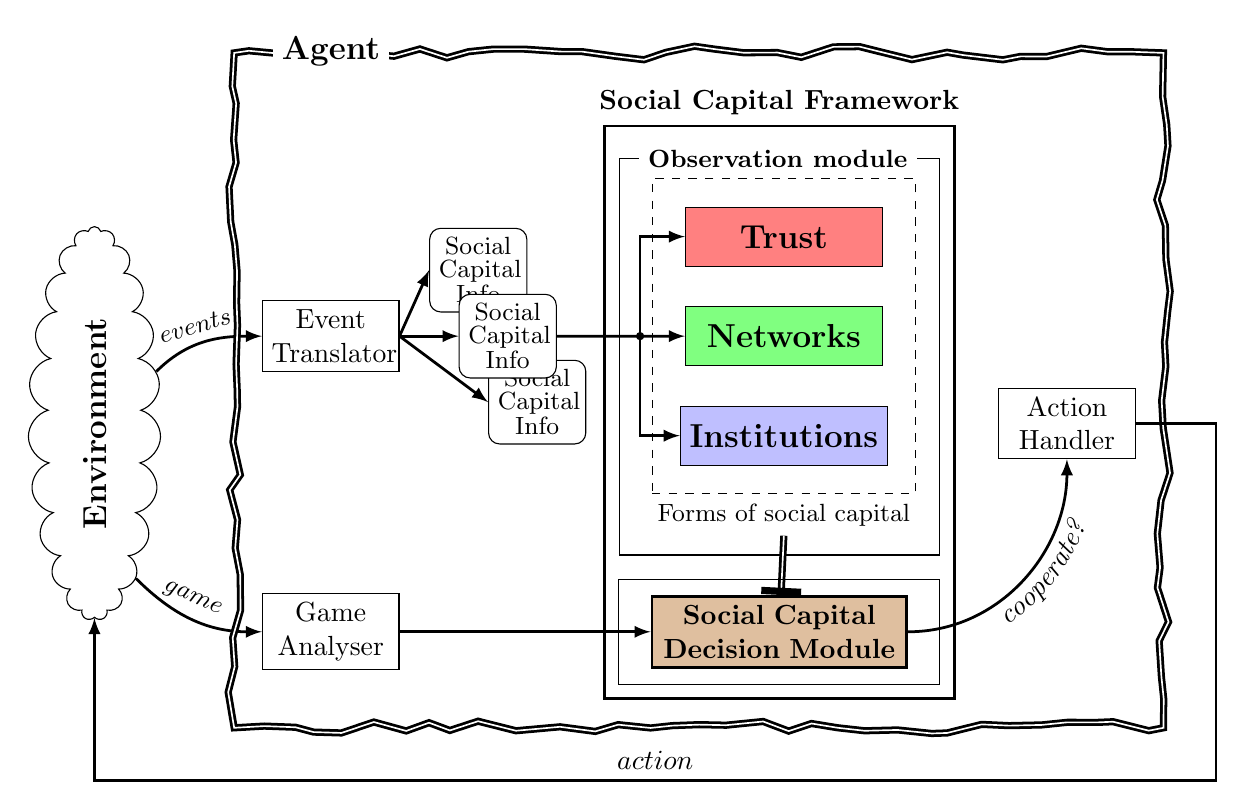
\begin{tikzpicture}

	% Styles
	\tikzstyle{scform} = [draw, minimum width=2.5cm, minimum height=.75cm]
	\tikzstyle{scinf} = [draw, minimum width=.75cm, minimum height=.75cm, text width=1cm,text centered,fill=white,rounded corners]
	\tikzstyle{lines} = [>=latex,line width=1pt]
	\tikzstyle{dot}=[circle,fill=black,minimum size=3pt,inner sep=0pt, outer sep=-1pt]

	% The 3 forms of SC
	\node [scform,fill=red!50] (tw) {\large \textbf{Trust}};
	\node [scform, below=.5cm of tw, fill=green!50] (net) {\large \textbf{Networks}};
	\node [scform, below=.5cm of net,fill=blue!25] (inst) {\large \textbf{Institutions}};
	
	% SC Information 
	\coordinate (scbase) at ([xshift=-2.25cm] net.west);
	\node [scinf, above left=.3cm and -.25cm of scbase] (sci2) {\small Social\\[-1mm]Capital\\[-1mm]Info};
	\node [scinf, below right=.3cm and -.25cm of scbase] (sci3) {\small Social\\[-1mm]Capital\\[-1mm]Info};
	\node at (scbase) [scinf] (sci1) {\small Social\\[-1mm]Capital\\[-1mm]Info};
	
	% Forms of SC container
	\node [fit={(tw) (inst)},draw,dashed,inner sep=10pt] (forms) {};
	\node [below=0cm of forms] (formslabel) {\small Forms of social capital};
	 
	% Edges SCI -> Forms of SC
	\draw [lines] (sci1) -- ($(sci1.east)!.65!(net.west)$) node[dot] (x) {};
	\draw [lines,->] (x.center) |- (tw);
	\draw [lines,->] (x.center) -- (net);
	\draw [lines,->] (x.center) |- (inst);

	% Update module container
	\node [draw,fit={(formslabel) (forms) (x)}, inner sep=7pt] (update) {};
	\node [above right=0cm and 0.25cm of update.north west, anchor=west,fill=white] (updateLabel) {\small \bf Observation module};	
	
	% Event translater node
	\node [draw,left=.75cm of sci1,text width=1.5cm,text centered] (trans) { Event\\Translator};
	
	% SC decision module
	\node [below=.5cm of update, draw, fill=brown!50,line width=1pt,text width=3cm,text centered] (scdm) {\bf Social Capital\\[0mm]Decision Module};
	
	% Edge update -> decision
	\draw [lines,->,-|,double] (formslabel.south) to (scdm);

	% Dummy coordinate at center
	\coordinate (mp) at ($(forms.north)!0.5!(scdm.south)$);
	
	% Environment
	\node at ([xshift=-3.cm] trans|-mp) [draw,cloud,aspect=0.5,cloud puffs=23,minimum width=1.5cm,minimum height=5cm,inner sep=-10pt] (env) {\rotatebox{90}{\large \textbf{Environment}}};

	% Edge env -> event translator
	\draw [lines,->] (env.40) to [in=180] node [above, sloped] {\small $events$~~} (trans.west);

	% Edge event translator -> SCI
	\draw [lines,->] (trans.east) -- (sci1.west);
	\draw [lines,->] (trans.east) -- (sci2.west);
	\draw [lines,->] (trans.east) -- (sci3.west);

	% Game analyser node
	\node [draw,text width=1.5cm,text centered] at (trans|-scdm) (game) { Game\\Analyser};
	
	% Edges env -> game analyser -> SCDM
	\draw [lines,->] (env.-75) to [out=-45,in=180] node [above, sloped] {\small $game$~~~} (game.west);
	\draw [lines,->] (game) to (scdm);
	
	% Dummy nodes and Container for decision module
	\node (decNW) at ([yshift=.2cm]update.west|-scdm.north) {};
	\node (decSE) at ([yshift=-.2cm]update.east|-scdm.south) {};
	\node [fit={(decNW.center) (decSE.center)}, inner sep=0pt,draw] (dec) {};
	
	% Container for SCFM
	\node [draw, line width=1pt, fit={(update) (dec) (updateLabel)}, inner sep=5pt] (scfm) {};
	\node [above=0cm of scfm] (scfmLabel) {\bf Social Capital Framework};
	
	% Action handler node
	\node [draw, right=2.75cm of mp,text width=1.5cm,text centered] (action) { Action\\Handler};

	% Agent container
	\node [draw, double, fit={(scfm) (trans) (action) (scfmLabel)}, inner sep=10pt, decorate, decoration={random steps}, line width=1pt] (agent) {};
	\node [above right=0cm and .5cm of agent.north west, anchor=west, fill=white] {\bf \large Agent};
	
	% Edges SCDM -> Action handler -> Env
%	\draw [lines,->] (scdm.east) to [out=0,in=-90] node [below, sloped] (coop) { {~~~$cooperate? ~[0..1]$}} (action);
	\draw [lines,->] (scdm.east) to [out=0,in=-90] (action);
	\draw [decorate,decoration={text along path,text={|\it|cooperate?},text align={center}},decorate] ([yshift=-0.3cm]scdm.east) to [out=0,in=-90] ([xshift=0.5cm]action);
	
	\draw [lines,->] (action) -| ([shift={(.65cm,-.65cm)}] agent.south east) -| node [above, near start] { $action$} (env);
	
	
\end{tikzpicture}

\end{document}